%
%
%First of all, TeXMakerX is now TeXStudio. If you are still running TeXMakerX then it is advised that you upgrade to the latest version of TeXStudio.
%
%minted uses Pygments of Python for the fancy coloring schemes. You need to invoke the -shell-escape option in order for LaTeX to allow Pygments to be used.
%
%In TeXStudio, click on the following menu
%
%    Options > Configure TeXStudio > Commands
%
%and change
%
%pdflatex -synctex=1 -interaction=nonstopmode %.tex
%
%into
%
%pdflatex -synctex=1 -interaction=nonstopmode --shell-escape %.tex
%
%Edit
%
%As mentioned by tohecz in comment, it is better to make a separate command for this in TeXStudio for security reasons. You can do this by clicking
%
%    Options > Configure TeXStudio > Build
%
%and in the User Commands box, click +Add button and add a name for your command in the first cell, say pdflatex -shell-escape and the command pdflatex -synctex=1 -interaction=nonstopmode --shell-escape %.tex in the second cell.
%
%You can then see the command listed in the menu
%
%    Tools > User
%
%Click on the command to run.

\documentclass[a4paper,11pt]{article}
\usepackage[T1]{fontenc}
\usepackage[utf8]{inputenc}
\usepackage{lmodern}
\usepackage[hidelinks]{hyperref} % Hyperref package for url's and [hidelinks] option to remove collouring
\usepackage{graphicx}
\usepackage{float}
\usepackage{listings}
\usepackage{minted}
%\title{}:
\title{Research Proposal UoM: a 3D Model of Neuroanatomical Abnormalities in Major Depressive Disorder}
\author{Russell Jarvis \\ Possible thesis advisor:  Tatiana Kameneva}

\usepackage{color}

\definecolor{mygreen}{rgb}{0,0.6,0}
\definecolor{mygray}{rgb}{0.5,0.5,0.5}
\definecolor{mymauve}{rgb}{0.58,0,0.82}

\lstset{ %
  backgroundcolor=\color{white},   % choose the background color
  basicstyle=\ttfamily\tiny,        % size of fonts used for the code
  breaklines=true,                 % automatic line breaking only at whitespace
  captionpos=b,                    % sets the caption-position to bottom
  commentstyle=\color{mygreen},    % comment style
  escapeinside={\%*}{*)},          % if you want to add LaTeX within your code
  keywordstyle=\color{blue},       % keyword style
  stringstyle=\color{mymauve},     % string literal style
}


\usepackage[utf8]{inputenc}

% Default fixed font does not support bold face
\DeclareFixedFont{\ttb}{T1}{txtt}{bx}{n}{12} % for bold
\DeclareFixedFont{\ttm}{T1}{txtt}{m}{n}{12}  % for normal

% Custom colors
\usepackage{color}
\definecolor{deepblue}{rgb}{0,0,0.5}
\definecolor{deepred}{rgb}{0.6,0,0}
\definecolor{deepgreen}{rgb}{0,0.5,0}

\usepackage{listings}

% Python style for highlighting
\newcommand\pythonstyle{\lstset{
language=Python,
basicstyle=\ttm,
otherkeywords={self},             % Add keywords here
keywordstyle=\ttb\color{deepblue},
emph={MyClass,__init__},          % Custom highlighting
emphstyle=\ttb\color{deepred},    % Custom highlighting style
stringstyle=\color{deepgreen},
frame=tb,                         % Any extra options here
showstringspaces=false            % 
}}


% Python environment
\lstnewenvironment{python}[1][]
{
\pythonstyle
\lstset{#1}
}
{}

% Python for external files
\newcommand\pythonexternal[2][]{{
\pythonstyle
\lstinputlisting[#1]{#2}}}

% Python for inline
\newcommand\pythoninline[1]{{\pythonstyle\lstinline!#1!}}


%\section{``In-text'' listing highlighting}


%\section{External listing highlighting}

%\pythonexternal{demo.py}

%\section{Inline highlighting}

%Definition \pythoninline{class MyClass} means \dots
\begin{document}

\maketitle
\tableofcontents


\section{Background}
Abnormalities in neuron and glial cell morphology have been observed in a range of brain pathologies including Major Depressive Disorder (MDD), autism, epilepsy, schizophrenia, and \cite{rajkowska2000postmortem}  \cite{brune2011neuroanatomical} \cite{snow2008altered} \cite{courchesne1997brainstem} \cite{sutula2002seizure} \cite{selemon1999reduced}. MDD and schizophrenia result in some overlapping structural abnormalities. In regards to schizophrenia these structural abnormalities include a net decrease in neuropil in the Pre Frontal Cortex (PFC) and parahippocampal gyrus \cite{selemon1999reduced} populations. In regards to MDD three types of neuro anatomical abnormalities have been observed: cell atrophy in the orbitofrontal cortex and dorsolateral PFC, cell death in the subgenual PFC, and increased densities of neurons in Anterior Cingulate Cortex (ACC) especially in Von Economo Neurons (VENs) cell populations \cite{brune2011neuroanatomical}. An increased density of neurons has also been observed in the hypothalamus and dorsal raphe nucleus \cite{rajkowska2000postmortem} populations.\\
\\
  %an increased density of Von Economo Neurons (VENs) in the  anterior cingulate cortex (ACC) \cite{brune2011neuroanatomical} has been noted. %Additionally metabolic changes have been identified in glial-neural units located in the ACC.\\ 
%\\
%During the past few years, the hypothesis of a complex metabolic abnormality in the ACC has been developed which links psychological abnormalities in MDD to abnormal baseline metabolism in astrocytes and neurons and even to disease related immunological processes in microglia (Dantzer et al., 2008)\\
%\\
The noted atrophy of neural trees and cell death has been attributed to several inter-related hypothesis pertaining to biochemistry in the brain. Firstly abnormal metabolic activity has been observed in neural-glial units in the ACC\cite{rajkowska2000postmortem}\cite{rajkowska1999morphometric}. Secondly it is believed that excessive levels of glucocorticoids hormones will be present in the MDD brain \cite{rajkowska2000postmortem} as a result of a poorly regulated hypothalamic–pituitary–adrenal system, and these glucocorticoids may be a major contributer to excito-toxic related neural atrophy and cell death \cite{sorrells2014glucocorticoids}. Thirdly MDD may also be a disorder of the genes coding for the neurotrophins associated with normal restorative brain plasticity \cite{dwivedi2010brain}, such that when excito-toxicity related atrophy of neurite occurs, the loss is less likely to be reversed by the growth of new neural material.\\
\\
The technique Resting State fMRI has implicated a hyper connected Default Mode Network (DMN) of individuals inflicted by MDD \cite{horn2010glutamatergic}\cite{liston2014default}, a result that is not intuitively obvious if one considers the reduced neuropil and infers reduced connection density as a consequence. However with regards to functional connectivity in the MDD brain what matters is the polarity of the remaining synapses and particularly how the ratio of excitatory to inhibitory projections is altered by selective excito-toxic pruning and cell death. Cognitive deficits involved in MDD may be caused by a reduced ability to inhibit a more hyper connected default mode network, as would be required to permit the engagement of task positive brain networks.\\ % anterior insular cortex (AI).\\ 
\\
Studies that apply combined fMRI and Proton NMR spectroscopy (MRS) to the study of Resting State Functional Connectivity (rsFC) are able to derive more specific information on the polarity of connectivity in the MDD and schizophrenic brain\cite{horn2010glutamatergic}. The availability of this new data type describing gross changes to synapse connection polarity is good news for $\mu$ circuit neural modellers who wish to create a more detailed structural-functional understanding of neural networks inflicted by MDD and schizophrenia.\\ 
\\
Although MDD and schizophrenia are both characterised by reduced neuropil in some overlapping structures, the illnesses are distinguishable across a range of neuroanatomical measures. DTI-MRI imaging has been used to distinguish between the MDD and schizophrenia in the female brain with a high success rate. Additionally DTI can distinguish between bipolar disease and MDD\cite{ota2013discrimination}.\\ %The physical expression of %schizophrenia in brain structures has a sexual dimorphic component.\\
\\
\section{Introduction}

This research proposal introduces simulation techniques intended to mimic salient neuro-anatomical abnormalities observed in MDD by way of a 3D structural and dynamic model. The model will include abnormal density of dendrite tree, and abnormal cell density in network models of appropriate brain regions, and abnormal ratios of excitatory and inhibitory neurotransmitters in order to try to create an in-silico replication overlapping MDD and schizophrenic brain conditions.\\ 
\\
By replicating attempting to model MDD neural substrate, methods proposed herein will facilitate an investigation into pathological dynamic neural activity. This modelling work should build the foundation to permit the future study of abnormal Evoked Potentials (EPs) and cognitive deficits that are present MDD subjects\cite{frodl2006reduced}\cite{sur2009event} via way of simulating approximate neural effects of TMS pulses. The modelling work should also provide a foundation for a detailed model of glial-neuron interactions in the MDD brain. Modelling methods presented herein are intended to act on accumulating publicly available data, and to build on pre existing modelling techniques.\\ 
\\
\section{Structure-Function Relationship in real Neurons and Neural Models}
Many large and medium scale neural network simulations neglect to model accurate 3D neuro anatomical structure \cite{kerr2012electrostimulation} \cite{neymotin2011synaptic} \cite{cutsuridis2010encoding}. Although large scale neural models including digitally reconstructed morphologies are more complex and harder to implement, in non electrotonically compact neurons, a neurons 3D form is a large determinate of its firing pattern \cite{mainen1996influence}. The ratio of neuron membrane surface to volume contributes to the neurons input impedance across a range of different frequencies and cell locations \cite{carnevale1997comparative}. In pyramidal neurons, neuron morphology distinctly determines neural firing pattern in addition to determining the connectivity between cells \cite{mainen1996influence}\cite{cuntz2011trees}\cite{branco2011synaptic}\cite{torben2008evol}.\\  
\\
%\section{Why Exclusive Rate coding in the entire brain is not feasible}
The researcher Cazé has asserted that computational capacity of a neuron is directly linked to the a its ability to perform a mapping of arbitrary input output transfer functions. If a neurons dendrites are able to compute the XOR function (a linearly non-separable function), then this signifies a neurons ability to perform a greater range of possible mappings. Cazé has demonstrated that in theory some types of neurons are able to solve the XOR function\cite{caze2013passive}.\\
\\
It has been hypothesised that different locations along the pyramidal neuron dendrite perform different types of encoding on inputs, with the distal dendrite spines performing coincidence detection encoding, and the proximal dendrite and somata performing rate en-coding \cite{branco2011synaptic}. It has also been hypothesised that each pyramidal neurons unique electro-physiology places it on a continuum between pure coincidence detection and pure temporal integration, neurons that lie between either extreme may be able to perform multiplexed rate and temporal encodings of their inputs, as described above.\\ 
\\
An encoding scheme based on a temporal averaging alone such as the firing rate code neglects all the information possibly contained in the exact timing of dendrite inputs, resulting in a decreased entropy rate of information that can be transferred from neuron to neuron, and thus decreasing the computational capacity related to inter neuron communication. This short coming of rate coding makes multiplexed rate and temporal coding theoretically attractive.\\
\\
It is generally a bad idea to build excessive complexity into models, since a good model is able to make accurate predictions via application of simplifying assumptions, however in the field of neuroscience there are several reasons to model neural networks by utilising as much of available morphological and 3D network topology information as possible.\\
\\
Firstly by trying to reconstruct neural circuits exclusively out of point model or abstract neurons, there is a risk of not properly representing the full computational capacity of each constituent neuron\cite{caze2013passive}, and as a consequence under representing the computational capacity of the entire network. Under representing the computational capacity of a neural network is of concern when the goal is to corroborate empirical findings of cognitive deficits in MDD and schizophrenia.\\
\\
Secondly by using 3D neuron morphologies in neural models, it is more possible to reproduce a natural model of multiplexed rate and temporal encoding in pyramidal neurons. Using brain derived digitally reconstructed cells to help facilitate a naturally occurring multiplexed encoding scheme is a second way to reduce the risk of under representing the information processing capacity of modelled brain regions involved in MDD.\\
 %of their dendrite inputs supporting a higher rate of information transmission between neurons. By using 3D morphology in neural network models 
%Suggesting that each neuron
 %A network wide simulation of neural pruning\\ 
\\
Thirdly in order to properly capture neuron circuit functionality, it is important to replicate neuron wiring in $\mu$ circuits under investigation. Although large variation in expressed neural wiring is an innate feature of the mammal brain, statistical regularities in wiring exist within mammal species, and it is arguable that some approaches to modelling 3D network topology are able to represent a better than random representation of rodent brain wiring, by utilizing measured statistical regularities of wiring within a specific species.\\
\\ %informed by available brain wiring statistics such as that given by the Allen Brain Mouse Connectivity Atlas.\\
Methods in this proposal aim to produce accurate connectivity, by using a sample of brain derived digitally reconstructed neurons to seed a neuro developmental algorithm that grows one or more forests of neuron trees, where the development of each tree is determined in relation to the development of other trees in the forest \cite{torben2014context}. After wiring the near contact points of these morphologies togethor, wiring quality can again be improved by revising the resulting  connectivity with statistics derived from Allen Mouse Brain Connectivity Atlas. A similar approach of using to neuron network building based on software generated artificial morphologies has been used before \cite{migliore2014distributed}, and its use may become increasingly routine.\\ 
\\
Fourthly it has been argued that cortical column neural circuits contain innate knowledge \cite{markram2011innate}. In modelling work by Neymotin a stream of stored synaptic information emitted by a network was measured using normalised transfer entropy \cite{neymotin2011synaptic}. Amongst electronically extended cells, variation in electrotonic length distributions across the neurons dendrite tree endows each neuron with its own unique input sensitivity and firing patterns. It could be argued that in addition to variations in wiring, variation in electrotonic parameters in neurons are representative of innate knowledge that can be emitted from the mammalian brain. Cell specific variability in firing times (rather than being merely noise), may instead represent complicated temporal spatio signals that may be reproduced and therefore recalled in the future.\\
\\
Fifthly it has been hypothesised that neural pruning is a normal feature of Slow Wave Sleep (SWS), and that SWS causes net synaptic downscaling of distal dendrite material representative of post synaptic weights such as dendrite spines \cite{tononi2003sleep}. A loss of distal dendrite tree may be combined with upscaling and strengthening of selective synapses which are substrate to salient memories, this combination of selective upscaling against a background of downscaling has been referred to as embossing \cite{ribeiro2012sleep}. It has also been hypothesised that regular circadian atrophy of neural tree also facilitates the clearance of toxic proteins by temporarily increasing the interstitial space available for transporting proteins \cite{mckinley2013don}. Insomnia and hypersomnia are common clinical features of severe to moderate depression. MDD is characterised by substantial changes to the timing of sleep related dynamic brain changes \cite{srinivasan2009pathophysiology}, and presumably to the architecture of brain networks that support sleep. A long term absence of synaptic downscaling due to accumulated sleep deprivation, may also contribute to hyper-excitability in some cell populations (due to reduced synaptic downscaling) \cite{sarasso2014quantifying}. However increased excitability may possibly lead to excito-toxicity in key neural populations and as well as a net increase to functional connectivity in the brain \cite{sarasso2014quantifying}. As far as I know it has not been theoretically tested if this periodic temporary loss of neurite tree contributes to the brain dynamics observed during SWS. It is testable whether a net decrease in distal dendrite subunits, and dendrite spines results in a net change in electrotonic compactness and electrical behaviour of all cells, such that collective firing dynamics are significantly altered. 
%Neural firing patterns are restrained by morphologies.\\ %Algorithms cause natural variability in the distribution of firing patterns, and input sensitivity of the neurons. The proposed approach to building a morphologically informed 3D neural network allows us to ask the question: What is the contribution of neuronal morphology to an intrinsic source of information emitted from the network.

%It can be argued that common human behaviour requires information stored in the brain to be synthesised with current sensory information in order for threatening and dangerous real world events to be acted on.  %\\ Kreutz spike distance can be used to find how desynchronized neural activity is.

 % Local Active Information. %information transmission, and the phase timing and sequence of excitatory neurons relative to an inhibitory population.%transformation?\\
%Exhaustive bivariate transfer entropy on the entire simulated network can be used 
%\\ %Such relationships can not be inferred a-proiri because of the complexity of the models, and often simulations can yield counter intuitive results.

%
\section{Testable Hypothesis}

%Conditional Mutual information is the same as transfer entropy.
%pdflatex -synctex=1 -interaction=nonstopmode --shell-escape %.tex
%Neural decoding.


% of the relationship between collective structural contributions of systematic atrophy, and overgrowth to measurable properties in the collective activity of neurons.

%occurs due to changes caused by . 
%\\ %The main hypothesis of this research is to examine whether reduced neuropil causes abnormal collective neural activity by means of a gross effect on electrotonic compactness of appropriate populations of neurons,  
% and overgrowth in appropriate cell populations. 

We want to find out about impaired cognitive functions, are relate this to reduced neuropil. Phase changes due to reduced neuropil. One signal arrives out of phase relative to another signal, so the two signals cannot be integrated with a coincidence detector.

If you have a matrix of bivariate transfer entropies (between one cell and every other cell), try to find out if the entropy in the spike train of one neuron, can be predicted by previous time steps of entropy in all the other neurons spike trains. Average the total indegree predictability of the neuron. Ie average how well the neurons spike train could have been predicted from all of the other neurons spike trains. Then find the LAIS in that neuron (find how well that neurons own past predicts its future (ie is its output regular and periodic?)). How well can a neuron be predicted from its own activity. 

I want to measure the computational capacity of neural networks. I think this is related to how much novel information it can create. This is related to how unpredictable the average signal is, this is related to the average transfer entropy indegree plus the average LAIS. If you took the inverse of this sum, the larger the number the more unpredictable the network would be and the less information they would be adding to the signal. The only problem with that is truly random signals are less predictable

The whole point of networked neurons, is they are coupled, ie they act less indipendently, they all influence each others activity. They all correlate with each others activity. Nevertheless some neurons will act more indipendently than all of the others, or also some neurons will be less predictable than the others.

A neuron may be more sensitive to its own internal feedback about its firing rate, than it is sensitive to external sources of feedback such as synaptic input.


There are many models which have been used to investigate structural-functional relationships in neuron morphology of a single neuron\cite{caze2013passive}\cite{carnevale1997comparative}\cite{Destexhe:2007}. Conversely there are many network scale models that seek to investigate the impact of systematic network wiring on the collective behaviour of uniform point model neurons\cite{kerr2012electrostimulation}\cite{neymotin2011synaptic}. The unique purpose of the proposed model is to euclidiate relationships between collective changes in variable non electrotonically compact single cell structure, to collective changes in the electrical activity of the neural populations, independently to changes in network wiring.\\
\\
As stated above the main hypothesis of this research proposal is that net electrotonic modification of cells corresponding to reduced neuropil results a measurable modification of the collective firing patterns of neurons. The goal of the proposed research is to examine what degree of neural pruning is required to cause a significant effect on collective neural activity and to separate any effect on collective neural activity from that which could be caused by abnormal wiring in reduced neuropil.\\
%find out if this putative effect causes pathological brain dynamics independently of the abnormal brain wiring that is also a consequence of reduced neuropil.\\
\\
This thesis can be tested using the network model described herein, by keeping neural connectivity constant, and iteratively pruning and growing appropriate forests of neurons to match MDD and schizophrenic brain conditions, in this way a threshold level of atrophy, such that beyond the threshold the network is no longer able to function via compensatory mechanisms.\\ %and neural networks can sustain can be discovered,
\\
Another (longer term) aim of the research is to corroborate findings about cognitive deficits in MDD and schizophrenia pertaining to abnormal EPs that have been observed\cite{sur2009event}, by using Local Field Potentials (LFPs) generated by this model and comparing them to Evoked Potentials observed in EEG\cite{frodl2006reduced}.\\
\\

%In brain networks that are inflected by MDD it would be useful to know what 

\section{Methods}

The methods can be divided into modelling techniques, and analysis techniques.

\subsection{Modelling Techniques}
Active neuron ion mechanisms should not be overly complicated, since what is intended is to test the hypothesis that varied neurite branching changes collective neuron firing dynamics, this hypothesis should remain true regardless of the accuracy of neuron firing dynamics.\\
\\
The requirements for building an in-silico biologically informed neural network model include data, and methods that act on the data. Currently there are many existing publicly available datum \cite{ascoli2007neuromorpho} and methods \cite{hines2009neuron} \cite{hines2008translating}\cite{migliore2014distributed}, developed in such a way as to encourage re-use and re-purposing. Many in-silico neural network models build on top of these existing approaches in a hierarchical manner, likewise the proposed research will also add extensions to already existing neural simulation foundations \cite{carnevale2006neuron}\cite{close}.\\
\\
%as some the foundations have to some extent already been layed. %By the NEURON simulation environment, and senselab.
The proposed approach to constructing a three dimensional neural network model of reduced neuropil brain conditions will involve lever-aging multiple publicly available neural datum from the rodent brain, and model building methods pertaining to both the structural and dynamic properties of in-silico neurons. Relevant data attributes include, digitally reconstructed cell morphologies (SWC files) \cite{ascoli2007neuromorpho}, cell centre coordinates, information about the presence and distribution of ion channels in target cells, presence and density of neuro transmitter mechanisms, neuron connectivity statistics. The methods include, synthetic neural development algorithms spatial wiring algorithms, statistically informed network wiring algorithms, and dynamic electrical simulation.\\
\\
Regarding data, and attributes, cell morphologies can currently be obtained programmatically via Python using the Allen Brain Atlas SDK. The Allen Brain Atlas SDK also includes methods, including an Abstract Model Description Language. NineML is another model Description language, that happily coexists with the Allen Brain SDK. There is also at least one Pythonic method used for measuring the LFP\cite{linden2013lfpy}.\\
\\ 
The Message Passing Interface (MPI) is a tool which can facilitate using the collective resources of many computers such that a model can be loaded which would exceed the capacity of of the memory of one computer. Methods for populating simulated neural substrate with NEURON+Python+MPI already exist, additionally some of the code-base from a 3D olfactory bulb model can be re-purposed \cite{migliore2014distributed}.
\\
%The proposed procedure for trying to answer the research question is depicted in flow chart form below.
\subsection{Mix and Match Approach}
Neuron Morphologies and Circuits (NeuroMaC) supports a mixed methodology growth rule \cite{torben2014context}. Realistically varying synthetic morphologies can be 'grown' in NeuroMaC, by seeding the space with several Digitally Reconstructed Cell (DRC) stained morphologies \cite{torben2014context}, and establishing a context, or a constricted space for context sensitive neurons to grow around and between. Statistics describing the spatial distribution of a collection of brain derived morphologies can also be used to inform artificial neuron growth rules \cite{torben2014context}.\\ %The context can be thought of as a kind of seemingly irregular scaffold to guide the growth of new neurons
\\
Synthetic neural development algorithms such as NeuroMAC and others can be combined with the tuned morphologically accurate rodent brain derived perisomatic models obtained from the Allen Brain Atlas database. A simulated region of neural tissue will be populated by morphologies grown in accordance to different methodologies, including inserting simple swc files, in order to mix and match. The result of combining various synthetic and brain derived morphologies will be a small forest of neurons representative of the microcircuits of interest. Other information latent in the Allen Brain Atlas database can be utilized in-order to facilitate time varying simulations, in the particular network and neural circuit of interest.\\
\\
 
%\newpage 
%Simulated TMS Evoked Potentials. 
%Reduced amplitude of mean membrane potential at key events.  
\section{Work Flow}
\begin{figure}[H]
\centering
\includegraphics[width=0.7\linewidth]{./Flow_chart_research_proposal}
\caption{}
\label{fig:Flow_chart_research_proposal}
\end{figure}
\begin{figure}[H]
\centering
\includegraphics[width=0.7\linewidth]{./Dynamic_simulation}
\caption{}
\label{fig:Dynamic_simulation}
\end{figure}

\begin{figure}[H]
\centering
\includegraphics[width=0.7\linewidth]{./Wiring}
\caption{}
\label{fig:Wiring}
\end{figure}
\begin{figure}[H]
\centering
\includegraphics[width=0.7\linewidth]{./Analysis}
\caption{}
\label{fig:Analysis}
\end{figure}


\begin{figure}[H]
\centering
\includegraphics[width=0.7\linewidth]{./Total_work_flow}
\caption{}
\label{fig:Analysis}
\end{figure}



\subsection{Wiring Algorithm}
\subsection{Parallel Wiring Algorithm}

In previous Bachelors and Masters thesis work, I have identified key parts of a parallel collision detection algorithm. Some important parts of it are presented below in a mixture of psuedo code and NEURON+Python+MPI. The algorithm assumes that existing code has already categorised neuron membrane subtypes into different presynaptic and postsynaptic sets and the result of this sorting are two complementary $SectionLists$. \\
\\
Presynaptic sets includes axons trees when they are present or otherwise just somas. Post synaptic sets include all or any of apical dendrites, basal dendrites and soma. The presynaptic (red) and postsynaptic (blue) $SectionLists$ corresponding to Digitally Reconstructed Cell morphologies are depicted  in figure 6 and 7 below.

\begin{figure}[H] %[scale=0.25]
\caption{Classified Membrane in Two Pyramidal Neurons with Post Synapses (Black)}
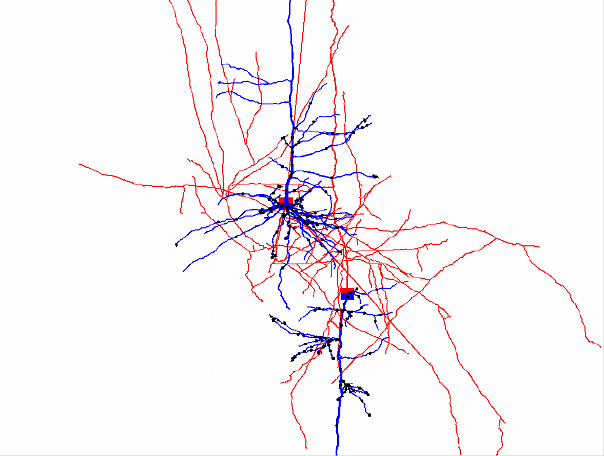
\includegraphics{classify}
\end{figure}%\$

\begin{figure}[H]
\caption{Classified Membrane in a Forest of Neurons}
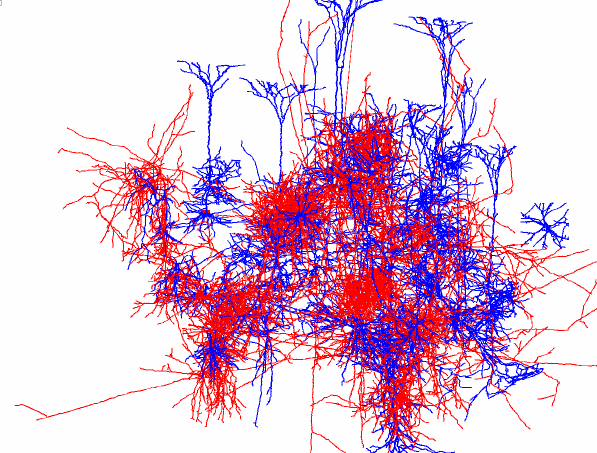
\includegraphics{pasted35}
\end{figure}

\newpage

% %
% Change font ot smaller.
% %

%\begin{lstlisting}[language=python, basicstyle= \small] 
%\begin{python}
\begin{minted}{python}
    def wirecells3(self):        
        '''wire cells between hosts, but don't wire cells on the same host.'''
        #def wirecells(RANK,NCELL,SIZE,h,icm,ecm):
        from segment_distance import dist3D_segment_to_segment
        import numpy as np
        NCELL=self.NCELL
        SIZE=self.SIZE
        COMM = self.COMM
        RANK=self.RANK
        icm = np.zeros((NCELL, NCELL))
        ecm = np.zeros((NCELL, NCELL))
        self.nclist=[]
        h=self.h    
        pc=h.ParallelContext()
        secnames = ''
        cellind =0 
        polarity = 0
        h('objref coords')
        h('coords = new Vector(3)')
        h('objref pc')
        h('pc = new ParallelContext()')        
 
        coordict=None
        coordictlist=None
        
    #Iterate over all CPU ranks, iterate through all GIDs (global 
    #identifiers, stored in the python dictionary).
        for s in xrange(0, SIZE):
            for j,l in self.celldict.iteritems():
                    
                                    
                if pc.gid_exists(j):
                    coordictlist=[]         

    #if the required GID is found on this CPU, get a reference to the cell
    #object and iterate through sections comprising its 
    #presynaptic tree (axonal).
                    
                    for sec in self.celldict[j].spk_trig_ls:
                        for seg in sec:
                            
                            
    #inside the Python HOC object 'h', the variable x_xtra denotes a
    #segment dependent x coordinate associated with a mechanism in the
    #section being iterated through, y and z coordinates can be obtained
    #via the same means.         

                            get_cox = str('coords.x[0]=x_xtra('
                                          + str(seg.x) + ')')

    #Use NEURONs self reflection to execute a string (data type), as an
    #instruction inside a call to the NEURON HOC object 'h'.                

                            
                            get_coy = str('coords.x[1]=y_xtra('
                                          + str(seg.x) + ')')
                            h(get_coy)
                            get_coz = str('coords.x[2]=z_xtra('
                                          + str(seg.x) + ')')
                            h(get_coz)
                            coordict={}
                            
                            secnames = sec.name()
                            cellind = int(secnames[secnames.find('Cell[') + 5:secnames.find('].')])

	#coordict is a dictionary that contains an array of coordinates, the GID of 
	#the putative presynaptic neuron, the segment of the putative 
	#presynaptic axon connection source and the section string name 
	#correspoding to the presynaptic location of those coorinates, this will all be
     #appended to a list which is updated in this nested for loop.
     
                            coordict['gid']=j 
                            coordict['seg']= seg.x
                            
                            secnames = sec.name()  # h.secnames                            
                            coordict['secnames'] = str(secnames)
                            coordict['coords'] = np.array(h.coords.to_python(),
                                              dtype=np.float64)
                            coordict['hostfrom']=RANK                  
                            #print i,j, ' i,j', seg.x, sec.name(), RANK
                                                
                            coordictlist.append(coordict)                  
     #Remove mechanisms, since the only point of these mechanisms, is to get accurate coordinates
     #once this has been achieved they can be uninserted from the spike trigger list.
                    h('uninsert xtra')
                    h('uninsert extracellular')
  
  	#After exiting the nested for loop broadcast those coordinates to all hosts/ranks other than the one currently on.           

                    data = COMM.bcast(coordictlist, root=s)  # ie root = rank
                                
                    h('objref coords2') 
                    h('coords2 = new Vector(3)')
             
                    if len(data) != 0:
                      for k in data:
    #For every coordinate thats received from a broadcast.
                         for i,t in self.celldict.iteritems():
    #For ever GID thats on this host (in the dictionary)                                                                               
                            if i in self.celldict.keys():
                                if int(t.gid1) != int(k['gid']):  # if the gids are not the same.
    #Rule out self synapsing neurons (autopses), with the condition 
    #pre GID != post GID 
    #If the putative post synaptic gid exists on this CPU, the reference 
    #to the corresponding cell object is the element 't' in celldict gid-> cell dictionary
    #Iterate through the post synaptic 
    #tree.                    
                            
                                    for sec in t.spk_rx_ls:
                                        h('objref cell1')
                                        h('cell1=pc.gid2cell('+str(i)+')')
                                        secnames = sec.name()
                                        cellind = int(secnames[secnames.find('Cell[') + 5:secnames.find('].')])  # This is the index of the post synaptic cell.
 
                                       for seg in sec:
                                            
                                            h(str('coords2.x[2]=') + str('z_xtra(')
                                              + str(seg.x) + ')')
                                            h(str('coords2.x[1]=') + str('y_xtra(')
                                              + str(seg.x) + ')')
                                            h(str('coords2.x[0]=') + str('x_xtra(')
                                            + str(seg.x) + ')')
        
                                            h('coordsx=0.0')
                                            h.coordsx = k['coords'][0]
                                            h('coordsy=0.0')
                                            h.coordsy = k['coords'][1]
                                            h('coordsz=0.0')
                                            h.coordsz = k['coords'][2]
                              
                                            coordsx = float(k['coords'][0])
                                            coordsy = float(k['coords'][1])
                                            coordsz = float(k['coords'][2])

    #Find the euclidian distance between putative presynaptic segments, 
    #and putative post synaptic segments.

    #If the euclidian distance is below an allowable threshold in micro 
    #meters, continue on with code responsible for assigning a 
    #synapse, and a netcon. Neurons parallel context class can handle the actual message passing associated with sending and receiving action potentials on different hosts.                               


                                            r = 0.
                                            import math
                                            r=math.sqrt((h.coords2.x[0] - coordsx)**2+(h.coords2.x[1] - coordsy)**2+(h.coords2.x[2] - coordsz)**2)
                                            gidn=k['gid']    
                                            r = float(r)
                                            if r < 10:  
    
                                                print r,# 'this is not hopefuly wiring everything to everything'
                                                polarity = 0        
                                                polarity=int(h.Cell[int(cellind)].polarity)
                                                print seg.x, k['seg'], k['secnames'], sec.name(), RANK, k['hostfrom'], k['gid'], int(h.Cell[int(cellind)].gid1)
                                                
                                                print polarity
                                                h('objref syn_')        
                                                if int(polarity) == int(0):
                                                    post_syn = secnames + ' ' + 'syn_ = new GABAa(' + str(seg.x) + ')'
                                                    icm[i][gidn] = icm[i][gidn] + 1
                                                else:
        
                                                    post_syn = secnames + ' ' + 'syn_ = new AMPA(' + str(seg.x) + ')'
                                                    ecm[i][gidn] = ecm[i][gidn] + 1
        
                                                h(post_syn)
                                                print post_syn
                                                h('print syn_')
                                                syn_=h.syn_
                                                h.syn_.cid=i
                                                h.Cell[cellind].ampalist.append(h.syn_)
                                                h.Cell[cellind].div.append(k['gid'])
                                                h.Cell[cellind].gvpre.append(k['gid'])
                                                nc=pc.gid_connect(k['gid'],syn_)                                        
                                                h.nc.delay=1+r/0.4
                                                h.nc.weight[0]=r/0.4    
                                                self.nclist.append(nc)
                                    h('uninsert xtra)                          
    # Remove the mechanism, since the only point of these mechanisms, is to get accurate coordinates
    # once this has been achieved they can be uninserted from the spike trigger list.
              
                                                        
            data=None                        
        ecm,icm = self.matrix_reduce(ecm,icm)
        return (self.nclist, ecm, icm)

\end{minted}
%\end{lstlisting}
%\\
%With time the implementation of parallel wiring could be made more elegant and efficient by subsituting for loops for list comprehensions generators and iterators.\\
%\\
%\begin{lstlisting}[language=python, basicstyle= \small] 
%def query_all_neurons():
%    '''
%    Return API queries about biophysical perisomatic_neurons.
%    Returns a list of well known file keys, but not yet properly formed URLs.
%    '''
%    instance=allensdk.api.api.Api('http://api.brain-map.org')
%    #Request only files associated with a model.
%    returned=allensdk.api.api.Api.retrieve_parsed_json_over_http(instance,'http://api.brain-map.org/api/v2/data/query.json?criteria=model::NeuronalModel')
%    bphys = [n for n in returned['msg'] if 'Biophysical' in n['name'] ]
%    sid=[ b['id'] for b in bphys ]
%    listwk = [ bp.get_well_known_file_ids(n) for n in sid ]
%    return listwk
%
%def retrieve_files(filename,wkfc,instance,working_directory=None):    
%    '''
%    Arguments: the file name and the well known file code, an instance of the Allen Brain API object.
%    Builds a well known file URL, and actually downloads and caches the files locally.    
%    '''    
%    wk=instance.construct_well_known_file_download_url(wkfc) 
%    instance.retrieve_file_over_http(wk,filename)    
%    return #files are cached on hard disk nothing to return
%    
%
%def get_all_files(instance,bphys):
%    #phys is a big list of dictionaries, that contains all of the different types of files you might be 
%    #interested in, the list of dictionaries needs to be traversed in order to download all of the files.
%    #Note that calling retrieve_files iteratively inside a list comprehension is
%    #sufficient to download all the requested files, and store them to the current working directory.
%    
%    [ retrieve_files(y,x,instance) for n in bphys for x,y in n['modfiles'].iteritems() ]
%    [ retrieve_files(y,x,instance) for n in bphys for x,y in n['morphology'].iteritems() ]
%    [ retrieve_files(y,x,instance) for n in bphys for x,y in n['fit'].iteritems() ]
%    [ retrieve_files(y,x,instance) for n in bphys for x,y in n['stimulus'].iteritems() ]    
%    for n in bphys:
%        bp.create_manifest(str(n['fit'].values()[0]),
%                           str(n['stimulus'].values()[0]),
%                           str(n['morphology'].values()[0]),
%                           [0,1,2,3,4,5])
%        print mp.manifest
%        manifest_path = os.path.join(os.getcwd(), str(n['morphology'].values()[0])+str(manifest.json))
%        with open(manifest_path, 'wb') as f:
%            f.write(json.dumps(mp.manifest, indent=2))
%
%
%bphys = query_all_neurons()   
%#Download everything, only do this if you have not downloaded everything already, as some files are large
%#and time consuming.
%get_all_files(instance,bphys)
%instance=allensdk.api.api.Api('http://api.brain-map.org')
%downloads = [ instance.construct_well_known_file_download_url(d) for d in bphys ]
%working_directory='neuronal_model'
%\end{lstlisting}
%
%\begin{lstlisting}[language=python, basicstyle= \small] 
%h('objref py')
%h('py = new PythonObject()')
%h('nrnpython("gidpop={}")') 
%#This checks that all cells have synapses and they are not just APcounts.                                                                                                      
%hocstring='''
%objref strobj \n
%strobj = new StringFunctions() \n
%objref py \n
%py = new PythonObject() \n
%nrnpython("strlist=[]") \n
%nrnpython("gidlist=[]") \n
%strdef cell \n
%for i=0, 50000000-1{ \n
%    if (pc.gid_exists(i)) { \n
%       sprint(cell,"%s",pc.gid2cell(i)) \n
%       py.strlist.append(cell) \n
%       py.gidlist.append(i) \n
%    } \n
%} \n
%nrnpython("gidstr=zip(strlist,gidlist)") \n
%'''
%h(hocstring)
%gidstr='gidstr'
%
%gidpop={}
%pickle.dump(gidstr,open("gidpop"+str(pc.id())+".p", "wb" ))
%pc.barrier()
%lsoftup=[]
%ncsize=len(h.NetCon)
%#make a list of tuples where each list element contains (srcid,tgtid,srcpop,tgtpop)
%for i in xrange(0,ncsize-1):
%    srcs.append(int(h.NetCon[i].srcgid()))
%    tgts.append(int(h.NetCon[i].postcell().gid))
%    srcind=int(h.NetCon[i].srcgid())
%    tgtind=int(h.NetCon[i].postcell().gid)
%    #print strlist[tgtind]==dic[tgtind], ' sanity check '
%    #add to list of tuples, netcon src, netcon tgt, src index, target index.
%    lsoftup.append((int(h.NetCon[i].srcgid()),int(h.NetCon[i].postcell().gid),dic[srcind],dic[tgtind]))
%    
%#pickle dump the list of tuples.
%pickle.dump(lsoftup, open( 'lsoftup'+str(pc.id())+'.p', 'wb' ))
%
%\end{lstlisting}


\subsection{Risk Management in the Network Building Approach}

\subsubsection{Checking Neuron Morphology}
The quality of DRCs obtained from the neuromorpho database is not always reliable, and it is necessary to check certain qualities in each cell. At least one algorithm exists for checking that the varying cable radius constituting dendrite and axonal neurite has biologically realistic values, such as would permit saltatory conduction. 


\subsubsection{Checking Network Topology}

Three possible outcome of network topology quality are envisaged:

\subsubsection{Best Case:} Both the neuronal activity and the wiring pattern; the connectivity between cells, is constrained by successfully applying wiring principles that mimic real neural development.
\subsubsection{Moderate case:} The network is randomly wired, this is already case for many published point Leaky Integrate and Fire (LIF) neuron models.
\subsubsection{Worst case:} The network wiring is constrained (the wiring is non random), however the wiring pattern deviates strongly from statistical regularities in real rodent neuroanatomy.\\
\\
In order to mitigate the risk of only achieving wiring of quality described by the moderate case the and the worst case A second pass revision of network wiring designed to capture statistical regularities observed in Allen Brain Mouse connectivity Atlas should mean that the neuron wiring is somewhere between the moderate case and the best case.\\
\\
Sporns describes two types of network hubs. A hub that exhibits high centrality in a community (or cell population), and provincial hubs, a provincial hub is a cell which connects together two or more cell populations \cite{sporns2011networks}.\\
\\
The neural network will be instantiated in the memory of many different computers, therefore to identify hub nodes MPI-aware network analysis algorithms will be applied to the simulated forest structure of neurons to identify the connection degree of nodes. Node centrality can be determined on the basis of In-degree, out-degree, and node centrality. %Once provincial hubs have been identified, a transfer function for that hub is obtained. The transfer finding a transfer function that maps a neurons simulated input dendritic spikes onto its spiking output.\\
\\
Structural analysis can be used as a type of sanity check of the connection rules which are applied above. Node centrality is a useful statistic because the acceptable ranges of in-degree and out-degree centrality are sometimes empirically estimated for different classes of cells.\\
\\

%cells, growing  but only to build smaller sized networks. 

\section{Analysis Techniques}
Analysis should be performed on the level of some single cells, and also on the level of the collective output of the neurons. The Local Active Information Storage (LAIS) framework can be used to test the working memory capacity of inidividual cells comprising the reconstructed network, and an average estimate working memory capacity of individual cells may be estimated in order to corroborate a reduced working memory capacity, corresponding to reduced neuropil condition \cite{lizier2012local}.\\ %Does multivariate LAIS estimation for networks exist yet?
\\
In addition to an expected deficit in working memory under reduced neuropil conditions. Reduced neuropil is also expected to result in impaired recall of long term memories as absent dendrite material can no longer translate a neural signal by systematic amplification and attenuation. The missing signal modifications corresponding to absent dendrite subunits may have otherwise acted as contributers to stored information recalled by the network.\\ 
\\
System identification techniques have allowed neuroscientists to model the behaviour of a neuron, by recording dendritic inputs, and axonal outputs and deriving a nonlinear transfer function that can map the inputs onto outputs\cite{caze2013passive}. Of interest in MDD is how much pruning, or atrophy can a neuron tolerate before that neuron is unable to use compensatory mechanisms to obey the same transfer function as it did under normal brain conditions.\\
\\

%decreased contribution to translation of a propogating neural spike times may caused by the missing influence of absent dendrite in systematically amplifying or attenuating the signal \cite{neymotin2011synaptic}. %stream of stored information corresponding to atrophied distal dendrite subunits.\\
%\section{Dynamic Analysis Methods}

%in the neural model where all neurons are stimulated with a weak applied external current clamp that approximates applied current perpendicular to the applied magnetic field pulse, 
\section{Future Work}
Also of interest in the collective neural output is the reduction in a neural networks ability to coordinate outputs from different specialised circuits, such that those signals can be integrated into a perceptual whole. To this end it may be possible to simulate a situation approximate of TMS evoked activations (although a lot of theoretical work needs to go into this area).\\
\\
Such an artificial TMS pulse could be used in combination with LFP recordings to check for decreased latencies, and phase changes in the signal. Subsequent to a simulated approximate TMS pulse LFP recordings will be performed in both the pathological and normal conditions, to check for characteristics of EPs, in attempt to corroborate empirical evidence about evoked potentials.\\
\\
Existing real life studies combining EEG and TMS in the conscious and unconscious brain have used applied TMS to particular areas of the brain, and examined the flow of electrical activity from the focus of stimulation\cite{sarasso2014quantifying}. It is unclear whether reduced neuropil conditions will increase or decrease the total time required for electrical signals to traverse through large areas of the simulated networks, while the condition of reduced neuropil should decrease synapse density, decreasing the number of all available paths through neural material,  indirectly decreasing the total number of shortest paths through the neural material. On the other hand decreasing synaptic density will also decrease horizontal\cite{lin2014polarity} and recurrent movement of signals through the network. Much of this recurrent pathways maybe GABAergic, contributing a dampening effect when it acts via inhibitory neurotransmitters. If pruning and cell death tips the balance of excitation and inhibition in favour of excitation then some signals may more quickly propagate through the network. Any changes to signal latencies may have an impact on cognitive processes that rely on sequential information processing in the brain. Where the relative timing of convergent inputs at a sequential stage are crucial to the proper functioning of the circuit.\\
\\
%On the other hand by removing intervening neurons via simulated cell death, extra synaptic delays associated with intervening neurons have also been removed.\\
%\\
\\
\section{Conclusion} 
MDD is sometimes described as an affective disorder, or mood disorder, however MDD, also has consequences in terms of cognitive functioning and information processing in the brain. I believe that emotional functioning is partially determined by distinct temporal spatial patterns of APs in the brain, and depression can be understood in terms of impaired dynamics of information bearing signals that result from the atrophy of neurons morphologies and neural networks. The para-hippocampal gyrus and prefrontal cortex are both strongly implicated in emotional processing, the atrophy of these two regions is likely to effect the integration information pertaining to higher level signals originating from these two different brain regions \cite{sarasso2014quantifying}
\cite{tononi1998consciousness}.\\
\\
This research proposal describes the motivation for and the methods used for in order to create a better understanding of the cognitive deficits and temporal events that are impacted by reduced neuropil associated with MDD. This and similar work may help to characterise a cause and effect relationships between network atrophy, abnormal affect and impaired information processing. Clarifying the precise effect of structural changes to neural dynamics, should help us to understand the most efficient interventions for restoring healthy brain structure and brain dynamics.\\

\bibliographystyle{IEEEtran}
\bibliography{mybibtexDB}


\end{document}

%
%A consequence of multiplexed encoding in dendrites, is that neurons that are post synaptic to pyramidal axonal Action Potentials (APs), may receive information created under any of three different encoding schemes \cite{ratte2013impact}.\\ 

%Multiplexed rate and temporal decoding may imply that decoding and encoding of information may occur at every neuron, a set of circumstances that would decrease information transfer, since information may be created and destroyed relative to each neuron. Under the right circumstances synchrony can be transferred from neuron to neuron. Sychronise firing when it occurs, may act as a universal neural code permitting the preservation of information as it moves through multiple neurons. It is possible that the brain contains both universal and adaptive neural codes.\\

%(as is often the case in LIF neurons)
